\documentclass[xcolor={dvipsnames}]{beamer}
\mode<presentation>{\usetheme{boxes}}
\usecolortheme{default}
\setbeamertemplate{navigation symbols}{}%remove navigation symbols

\setbeamerfont{frametitle}{size=\Large}

%\setbeamercolor{structure}{fg=beamer@blendedblue}



\setbeamertemplate{bibliography item}{\insertbiblabel}

\setbeamercolor{bibliography entry author}{fg=black}
\setbeamercolor{bibliography entry title}{fg=black} 
\setbeamercolor{bibliography entry location}{fg=black} 
\setbeamercolor{bibliography entry note}{fg=black}  

\usepackage[style=numeric,sorting=ydnt,maxnames=1,defernumbers=true, firstinits=true]{biblatex}
\renewbibmacro{in:}{}
\ExecuteBibliographyOptions{sorting=ydnt}

%\addbibresource{./jlescSummerSchool_checkpointing.bib}

\makeatother
\setbeamertemplate{footline}
{
  \leavevmode%
  \hbox{%
    %% \begin{beamercolorbox}[wd=.2\paperwidth,ht=2.25ex,dp=1ex]{date in head/foot}%
    %%   \usebeamerfont{date in foot}
    %% \end{beamercolorbox}%
  %%   \begin{beamercolorbox}[wd=.6\paperwidth,ht=2.25ex,dp=1ex, center]{date in head/foot}%
  %%     \usebeamerfont{date in foot}\insertshortdate
  %% \end{beamercolorbox}%
  \begin{beamercolorbox}[wd=\paperwidth,ht=2.25ex,dp=1ex]{date in head/foot}%
    \usebeamerfont{date in foot}\hfill
    {\scriptsize\insertframenumber{}}\hspace*{2ex}
  \end{beamercolorbox}}%
  \vskip0pt%
}
\makeatletter



\usepackage[utf8]{inputenc}
%\usepackage[T1]{fontenc}
%\usepackage[francais]{babel}
\usepackage{hyperref}
\usepackage{url}
\usepackage{pifont}
\usepackage{changepage}
\usepackage{listings}
\lstset{basicstyle=\ttfamily,
  showstringspaces=false,
  commentstyle=\color{black},
  keywordstyle=\color{black}
}

\usepackage{fancyvrb}
\usepackage{multirow}
\usepackage{tabu} 
\usepackage{colortbl}

\usepackage{marvosym}

\usepackage{eurosym}

%\usepackage{gitdags}
\usepackage{comment}

\usepackage{pdfpages}
\setbeamercolor{background canvas}{bg=}


\usepackage{perpage} %the perpage package
\MakePerPage{footnote}



\definecolor{beamer@blendedblue}{RGB}{0,102,204}

\definecolor{beamer@lightgray}{RGB}{238,238,224}


\definecolor{itemorange}{RGB}{255,114,0}


\definecolor{myorange}{RGB}{255,103,0}


\setbeamertemplate{itemize items}[circle]
\setbeamertemplate{itemize subitem}[triangle]


\setbeamercolor{itemize item}{fg=beamer@blendedblue}
\setbeamercolor{itemize subitem}{fg=gray}


\newcommand<>{\Blue}[1]{{\color#2{beamer@blendedblue}#1}}
%\newcommand<>{\Orange}[1]{{\color#2{BurntOrange}#1}}
\newcommand<>{\Orange}[1]{{\color#2{myorange}#1}}
\newcommand<>{\Alert}[1]{{\Orange{\textbf{#1}}}}


\newcommand{\largeskip}{\vspace{0.6cm}}
\newcommand{\hugeskip}{\vspace{1cm}}



\usepackage{tikz}
\usetikzlibrary{%
decorations.pathreplacing,%
decorations.pathmorphing,%
decorations.shapes,%
decorations.text,%
decorations.markings,%
shapes,%
shapes.callouts,%
shadows,%
arrows,
calc,%
positioning,%
chains,%
backgrounds,%
fit, %
fadings}

\tikzset{
    invisible/.style={opacity=0},
    visible on/.style={alt={#1{}{invisible}}},
    alt/.code args={<#1>#2#3}{%
      \alt<#1>{\pgfkeysalso{#2}}{\pgfkeysalso{#3}} % \pgfkeysalso doesn't change the path
    },
}


\tikzset{
    colornode/.style={
        outer sep=0pt, fill=#1!67, %text height=2ex, text depth=.5ex
    },
    cpu/.style={
        diamond, fill=gray!30, aspect=3, name=CPU#1,
        node contents={$\text{CPU}_{#1}$},
    },
    thread/.style={fill=#1!67,
        minimum width=5ex, minimum height=1.25em},
    tick/.style={very thin},
}



\newcommand{\email}[1]{\href{mailto:#1}{\nolinkurl{#1}}}

\newcommand{\xmark}{\ding{55}}


\AtBeginPart{
  %\frame{\partpage}
  \frame{
    \frametitle{Agenda}
    \small
    \tableofcontents[part=\insertpartnumber,
    sectionstyle=show,
    subsectionstyle=hide,
    subsubsectionstyle=hide]
  }
}

\AtBeginSection[]
{
  \begin{frame}
    \frametitle{Agenda}
    \small
    \tableofcontents[
    sectionstyle=show/shaded,
    subsectionstyle=show/show/hide,
    subsubsectionstyle=hide]
  \end{frame}
}

\AtBeginSubsection[]{
  \mode<presentation>{
    \frame{\tableofcontents[
      sectionstyle=show/hide,
      subsectionstyle=show/shaded/hide,
      subsubsectionstyle=show/show/hide]
    }
  }
}


\date[\the\year]{\the\year}

\newcommand{\shellcmd}[1]{\indent\indent\texttt{\footnotesize\$ #1}}


\title[]{Cloud Computing}
\subtitle{Définitions et concepts\footnote{Adapté du support développé par Thomas ROPARS et Renaud LACHAIZE}}

%Thomas ROPARS : \url{https://tropars.github.io/teaching/},
%\url{https://roparst.gricad-pages.univ-grenoble-alpes.fr/cloud-tutorials/m2gi-devops/}}}


\author[]{\\Danilo Carastan dos Santos
  \\ \vspace{0.5cm} \email{danilo.carastan-dos-santos@univ-grenoble-alpes.fr}}

\definecolor{mybrown}{RGB}{205,133,63}
\definecolor{myblue}{RGB}{28,134,238}

\let\Red=\alert
\newcommand<>{\green}[1]{{\color#2{green!70!black}#1}}
\newcommand<>{\blue}[1]{{\color#2{blue!100!black!100}#1}}
\definecolor{darkgreen}{rgb}{0,0.5,0}

\newcommand\myvdots{{\smash[b]\strut\smash[t]\vdots}}


\usepackage{boxedminipage}
\newenvironment{boitecode}[1]{
    \begin{boxedminipage}{\linewidth}      
%\begin{beamerboxesrounded}[shadow=true,lower=lightex,upper=medex]{#1}
    #1
    \begin{semiverbatim}
}{   \end{semiverbatim}\vspace{-1.5\baselineskip}
    \end{boxedminipage}
%  \end{beamerboxesrounded}
}


\begin{document}


\begingroup
\setbeamercolor{titlelike}{bg=beamer@lightgray, fg=black}
\begin{frame}
\titlepage
\end{frame}
\endgroup

\begin{frame}{Question de départ}
    \begin{center}
        \textbf{Selon vous, comment peut-on qualifier le Cloud Computing ?}
    \end{center}
\end{frame}

\begin{frame}{Une définition de Cloud Computing}
    Définie par le NIST :  \textit{National Institute of Standards and
    Technology
    (USA)\footnote{\url{http://nvlpubs.nist.gov/nistpubs/Legacy/SP/nistspecialpublication800-145.pdf}}}

    \vspace{5mm}

    \begin{block}{Définition}
    \textit{``Cloud computing is a model for enabling ubiquitous, convenient,
    \textcolor{red}{\textbf{on-demand}} network access to a
    \textcolor{blue}{\textbf{shared pool of configurable computing resources}}
    (e.g., networks, servers, storage, applications, and services) that can be
    \textcolor{orange}{\textbf{rapidly provisioned and released}} with minimal management effort or service
    provider interaction. %This cloud model is composed of \textbf{five essential
    %characteristics, three service models, and four deployment models.}''
    }
    \end{block}
\end{frame}

\begin{frame}{Shared pool of configurable computing resources}{Ensemble partagé de ressources informatiques configurables}
    \textbf{Idée :} louer un certain montant de capacité de calcul d'un data-centre physique.
    
    \vspace{5mm}
    \centering 
\includegraphics[width=.6\textwidth]{Figures/data-center-cloud.pdf}
\end{frame}

\begin{frame}{On-demand access}{Accès à la demande}
    \textbf{Idée :} J'ai besoin de ressources informatique (serveurs). J'accède un site
    web pour louer de serveurs (virtuelles). Je paye le temps d'utilisation.
    Tout est automatique.
    
    \vspace{5mm}
    \centering 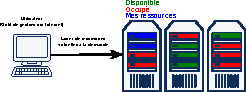
\includegraphics[width=\textwidth]{Figures/data-center-cloud-user.pdf}
\end{frame}

\begin{frame}{Rapidly provisioned and released}{Rapidement approvisionné et libéré} 
  \textbf{Idée :} Je n'ai plus besoin de ressources informatique (serveurs). Je demande
  la libération de ressources. Les ressources sont libérées.

  \vspace{5mm}
  \centering 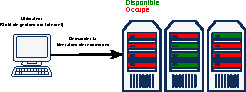
\includegraphics[width=.9\textwidth]{Figures/data-center-cloud-user-release.pdf}
\end{frame}

\begin{frame}{Concept clé : Virtualisation}

  Largeur des rectangles $\rightarrow$ demande de ressource (nombre de CPUs, quantité de mémoire, etc.)
  \vspace{5mm}

  \centering 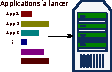
\includegraphics[width=.9\textwidth]{Figures/data-center-virt-1.pdf}  
  
\end{frame}

\begin{frame}{Concept clé : Virtualisation}

  \textbf{Sans virtualisation} $\rightarrow$ seulement une app par machine $\rightarrow$ ressources sous-utilisées
  \vspace{5mm}

  \centering 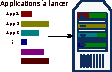
\includegraphics[width=.9\textwidth]{Figures/data-center-virt-2.pdf}  
  
\end{frame}

\begin{frame}{Concept clé : Virtualisation}

  \textbf{Avec virtualisation} $\rightarrow$ plusieurs apps par machine $\rightarrow$ meilleure utilisation de ressources
  \vspace{5mm}

  \centering 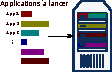
\includegraphics[width=.9\textwidth]{Figures/data-center-virt-3.pdf}  
  
\end{frame}

\begin{frame}{Types d'infrastructures Cloud}

  \textbf{Cloud Privé} 

\begin{itemize}
  \item Infrastructure utilisée \textbf{exclusivement} par une organisation
  \item Mode d'opération typique avant le cloud public
  \item Toujours pertinent (exemple : données sensibles) 
\end{itemize}

\centering 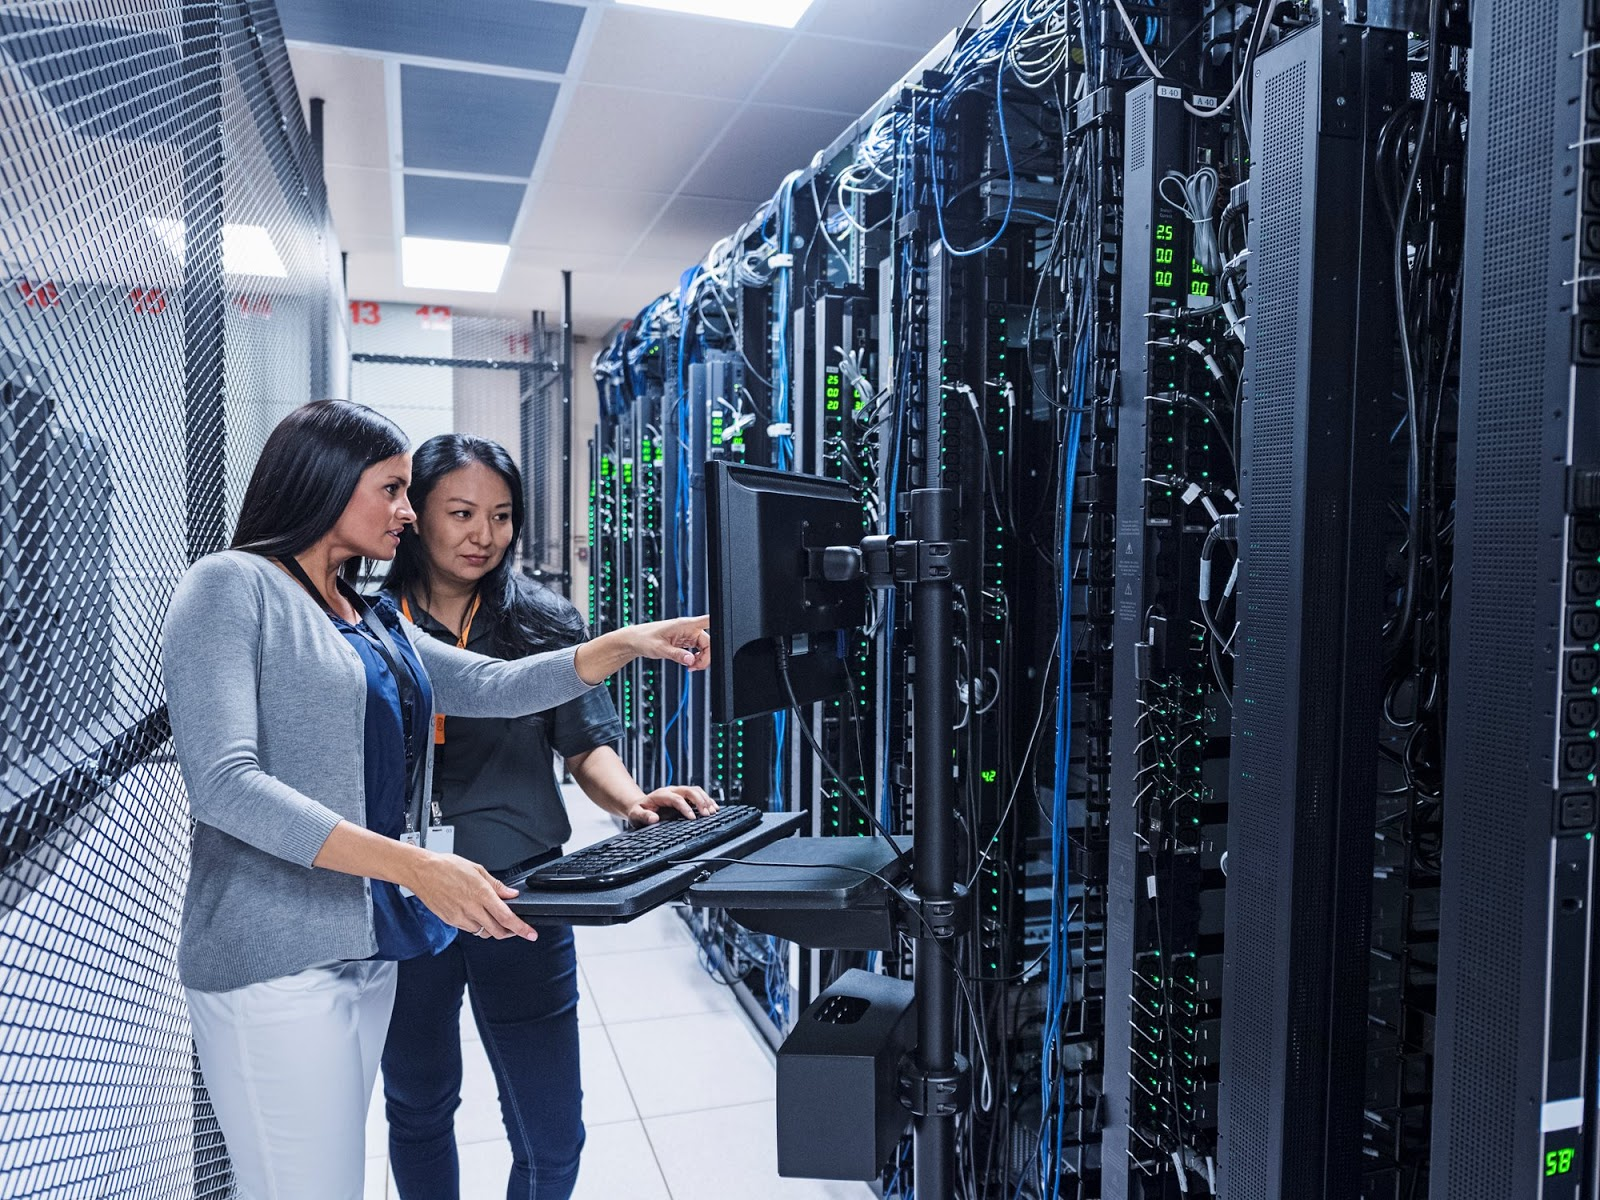
\includegraphics[width=.75\linewidth]{Figures/data-center.jpg}
  
\end{frame}

\begin{frame}{Types d'infrastructures Cloud}

  \textbf{Cloud Public} 

\begin{itemize}
  \item Infrastructure disponible au \textbf{grand public} (qui veut payer pour
  le service) par des fournisseurs de services cloud  
  \item Chaque client a un sous-ensemble isolé de ressources
  \item Infrastructure multilocataire   
\end{itemize}

\vspace{5mm}

\centering 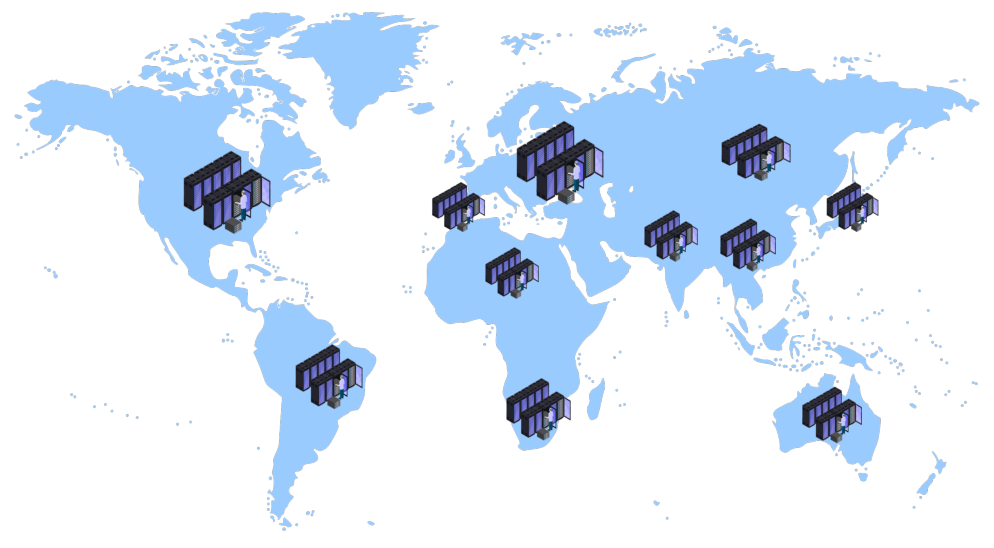
\includegraphics[width=.9\linewidth]{Figures/data-center-world.pdf}
  
\end{frame}

\begin{frame}{Types d'infrastructures Cloud}

  \textbf{Cloud Hybride} 

\begin{itemize}
  \item Un mélange entre le Cloud privé et le Cloud public
  \item Intérêt : 
  \begin{itemize}
    \item Augmenter la capacité du Cloud privé avec le Cloud public
    \item Flexibilité en fonction de chaque application (exemple : donnés
    sensibles $\rightarrow$ Cloud privé, sinon $\rightarrow$ Cloud public)
  \end{itemize}
\end{itemize}

  \textbf{Multi Cloud}

  \begin{itemize}
    \item Utiliser plusieurs fournisseurs de Cloud public
    \item Intérêt : Exploiter les avantages de chaque fournisseur en
    fonction du contexte de chaque application
  \end{itemize}
  
\end{frame}

\begin{frame}{Les Hyperscalers}

  \begin{itemize}
    \item Fournisseurs Cloud à très grande échelle 
    \item \textbf{Amazon AWS, Google Cloud, Microsoft Azure} 
    \item Des infrastructures titanesques\footnote{\url{https://youtu.be/80aK2\_iwMOs}} \footnote{\url{https://youtu.be/j07V-P7-MBo}}
  \end{itemize}

  \centering 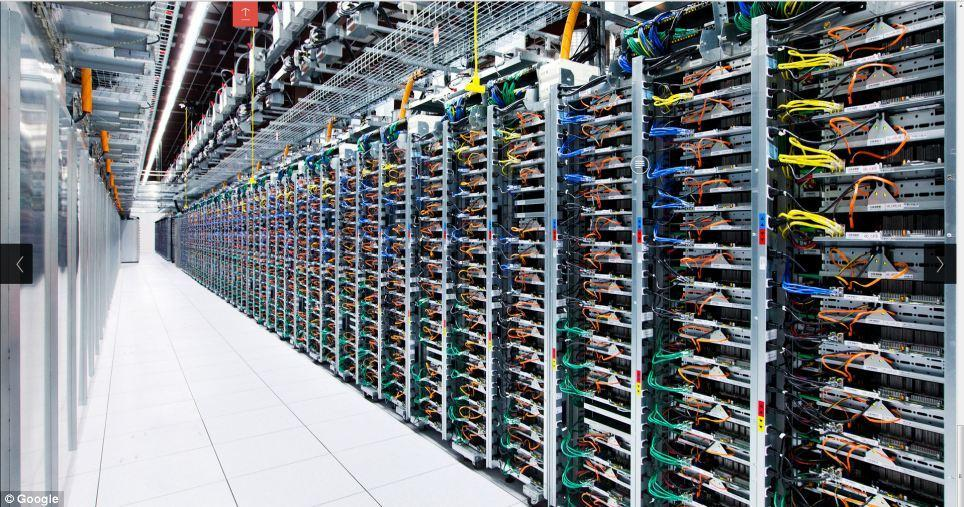
\includegraphics[width=.9\linewidth]{Figures/data-center-hyperscale.jpg}
  
\end{frame}

\begin{frame}{Les services Cloud}

  \begin{center}
    {\LARGE \textit{``X as a service''}}
    
    X en tant que service
  \end{center}

  \begin{itemize}
    \item Un certain service (X) qui est géré par un fournisseur Cloud
    \item Une centaine de services par chaque Hyperscaler. Chaque service a un nom différent\dots
    \item Liste de services :
    \footnote{\url{https://www.techtarget.com/searchcloudcomputing/feature/A-cloud-services-cheat-sheet-for-AWS-Azure-and-Google-Cloud}}
  \end{itemize}

  \textbf{Modèles de services Cloud} : Hiérarchie croissante de sous-traitance de contrôle et responsabilité. 

  \begin{itemize}
    \item \textit{Infrastructure as a service} : Infrastructure en tant que service
    \item \textit{Platform as a service} : Plate-forme en tant que service
    \item \textit{Function as a service} : Fonction en tant que service
    \item \textit{Software as a service} : Logiciel en tant que service
  \end{itemize}
  
\end{frame}

\begin{frame}{Infrastructure as a service (IaaS)}{Infrastructure en tant que service}
  \begin{itemize}
    \item Louer une infrastructure virtuelle 
    \begin{itemize}
      \item processeur, mémoire, stockage, réseau 
    \end{itemize}   
    \item Le fournisseur gère l'Infrastructure physique. L'utilisateur gère l'infrastructure virtuelle
    %\item Pratique pour déployer d'applications ``faite maison''
    \item Utilisateurs sont administrateurs système 
    \begin{itemize}
      \item Installer/configurer/gérer les mises à jour de sécurité : le système
      d'exploitation, serveur web, base de données, etc      
    \end{itemize}
    \item Exemple : Google Compute Engine\footnote{\url{https://cloud.google.com/compute}}
  \end{itemize}
\end{frame}

\begin{frame}{Platform as a service (PaaS)}{Plate-forme en tant que service}
  \begin{itemize}
    \item Louer une infrastructure virtuelle plus la maintenance des logiciels
    nécessaires pour l'application
    \begin{itemize}
      \item processeur, mémoire, stockage, réseau, serveur web, système de base
      de données
    \end{itemize}
    \item Utilisateurs sont développeurs
    \begin{itemize}
      \item Le fournisseur Cloud gère l'infrastructure (exemple : mise à jour du
      système d'exploitation, serveur web, système de base de données)
    \end{itemize}
    \item Exemples : Google Cloud
    Run\footnote{\url{https://cloud.google.com/run}} et App
    Engine\footnote{\url{https://cloud.google.com/appengine}}
  \end{itemize}
\end{frame}

\begin{frame}{Software as a service (SaaS)}{Logiciel en tant que service}

  \begin{itemize}
    \item Logiciel (application) complètement développe et accessible pour les utilisateurs à
    partir d'un navigateur    
    \item Il suffit d'avoir un navigateur connecté à l'Internet pour utiliser l'application
    \item Presque tout est transparent à l'utilisateur
    \begin{itemize}
      \item Gestion de l'infrastructure, logiciels nécessaires (serveur web,
      etc) et développement de l'application
    \end{itemize}    

    %\item La forme la plus simple de Cloud Computing
    \item Les utilisateurs ont très peu de contrôle (exemple : localisation des
    données, contrôle de latence de communication, etc)
    \item Exemples : Microsoft Office 365, Google Drive, Google Meet
  \end{itemize}

\end{frame}

\begin{frame}{Function as a service (FaaS)}{Fonction en tant que service}
\begin{itemize}
  \item Aussi mentionné comme \textit{Serverless Computing}
  \item L'application est développée comme plusieurs fonctions
  \begin{itemize}
    \item Chaque fonction attend qu'un événement se déclenche
    \item Une fois déclenchée, la fonction s'exécute. L'infrastructure et la
    plate-forme sont gérées par le fournisseur
    \item L'utilisateur ne paye que le temps d'exécution de la fonction    
  \end{itemize}
  \item Nécessite une façon spécifique de développer les applications
  (Microservices)
  \item Exemple : Amazon AWS Lambda\footnote{\url{https://aws.amazon.com/lambda/}}
\end{itemize}
  
\end{frame}

\begin{frame}{An avertissement sur les technologies Cloud modernes}
  \begin{itemize}
    \item Nous sommes actuellement submergés par des technologies
    \item Il faut choisir les technologies avec parcimonie, pour éviter de
    développer d'applications trop complexes sans nécessité
    \begin{itemize}
      \item Exemple : \textit{ A majority of real-world analytic jobs process less than 100GB of input data. For many of such
    jobs, a single ``scale-up'' server (i.e., a mid-range multicore server) can do as well or better than a
    cluster in terms of performance, cost, power and server density.\footnote{[R. Appuswamy et al. “Nobody ever got fired for buying a cluster”. 2013.]}}
      \item Plus d'exemples: \url{https://blog.bradfieldcs.com/you-are-not-google-84912cf44afb}
    \end{itemize}
  \end{itemize}
\end{frame}

\begin{frame}{An avertissement sur les technologies du numérique}  
  La sur-numérisation peut aussi desservir
  \begin{itemize}
    \item Exemple : Commentaire de Yassine Lakhnech sur l'allongement des
    délais de traitement de titres de séjour d'étudiants à
    l'UGA\footnote{\url{https://mesinfos.fr/38000-grenoble/universite-grenoble-alpes-si-la-securite-n-est-plus-garantie-on-sera-obliges-de-demenager-206296.html}}
    \item "Ça fonctionnait très bien à Grenoble, mais la dématérialisation a
    fait que la situation se détériore. La disparition des accueils physiques
    a provoqué une forme de rigidité. On peut blablater sur l'attractivité
    internationale, mais si les étudiants et les chercheurs se retrouvent sur
    le coup d'une OQTF, et ne peuvent plus rentrer chez eux à Noël sous peine
    de ne pas pouvoir revenir, ça n'a pas de sens".
  \end{itemize} 

\end{frame}

\end{document}